\documentclass[12pt, a4]{article}
\usepackage[english]{babel}
\usepackage[utf8x]{inputenc}
\usepackage{fullpage}
\usepackage{listings}
\usepackage{graphicx}
\usepackage{color}

%Syntax highlighting
\definecolor{blue-violet}{rgb}{0.54, 0.17, 0.89}
\definecolor{ao}{rgb}{0.0, 0.5, 0.0}
\definecolor{amaranth}{rgb}{0.9, 0.17, 0.31}
\definecolor{ballblue}{rgb}{0.13, 0.67, 0.8}
\definecolor{onyx}{rgb}{0.06, 0.06, 0.06}


\lstset{
  breaklines=true,                 % automatic line breaking only at whitespace
  captionpos=b,                    % sets the caption-position to bottom
  breakatwhitespace=false,
  keepspaces=true,
  numbers=left,
  numbersep=5pt,
  showspaces=false,
  showstringspaces=false,
  showtabs=false,
  tabsize=4,  
  backgroundcolor=\color{white},   % choose the background color
  commentstyle=\color{ao},    % comment style
  keywordstyle=\color{amaranth},    % keyword style
  stringstyle=\color{blue-violet},    % string literal style
  numberstyle=\tiny\color{ballblue},	   % number style
  basicstyle=\ttfamily\footnotesize\color{onyx} % size of fonts used for the code
}

%Document Header
\title{\textbf{Department of CSE\\SSN College of Engineering}}
\author{\textbf{Vishakan Subramanian - 18 5001 196 - Semester VII}}
\date{27 October 2021}

\begin{document}
\maketitle
\hrule
\section*{\center{UCS 1712 - Graphics And Multimedia Lab}}
\hrule
\bigskip

%Assignment Details
\subsection*{\center{\textbf{Exercise 10: Creating a 3D Scene in C++ using OpenGL}}}
\subsection*{\flushleft{Aim:}}
\begin{flushleft}

Write a C++ program using OpenGl to draw atleast four 3D objects. Apply lighting and texture and render the scene. Apply transformations to create a simple 3D animation. 
\bigskip

\textbf{OpenGL Functions to use:}

\begin{itemize}
	\item glShadeModel()
	\item glMaterialfv()
	\item glLightfv()
	\item glEnable()
	\item glGenTextures()
	\item glTexEnvf()
	\item glBindTexture()
	\item glTexParameteri()
	\item glTexCoord2f()
\end{itemize}

\bigskip
\textbf{Note:} Use built-in transformation functions.
 
\end{flushleft}

%Code
\newpage
\subsection*{\flushleft{Code: 3D Scene:}}
\begin{flushleft}
\lstinputlisting[language = C++]{Animations.cpp}
\end{flushleft}


%Output
\newpage
\subsection*{\flushleft{Output: Scene - 1}}
\begin{figure}[h]
\centering
\caption{Scene - 1.}
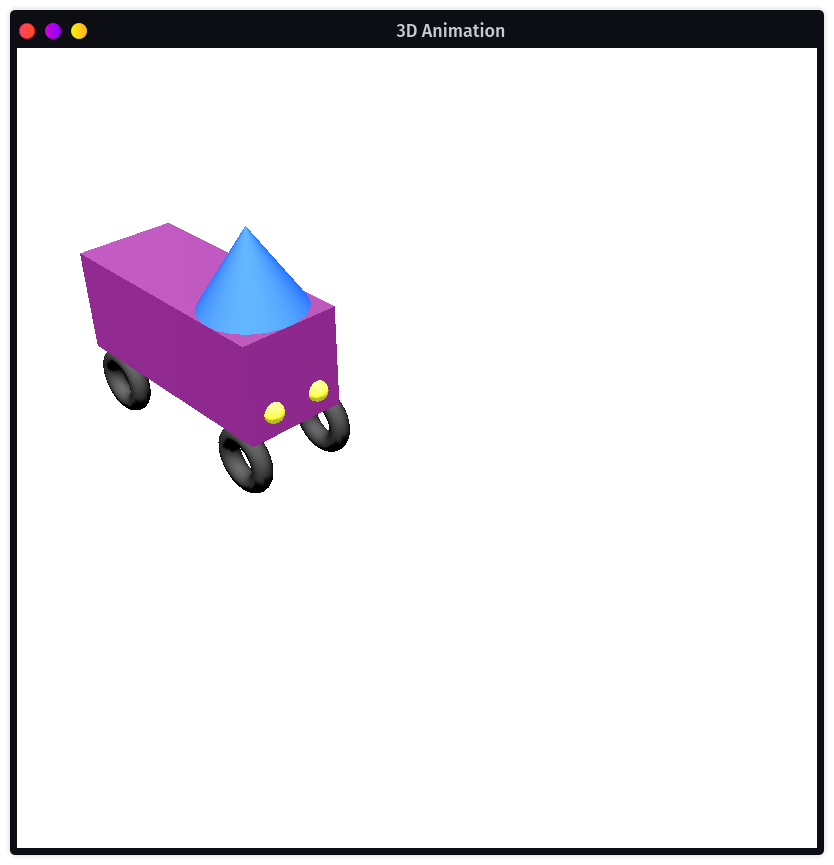
\includegraphics[height=15cm, width=15cm]{Outputs/Animation-0.png}
\end{figure}

\newpage
\subsection*{\flushleft{Output: Scene - 2}}
\begin{figure}[h]
\centering
\caption{Scene - 2.}
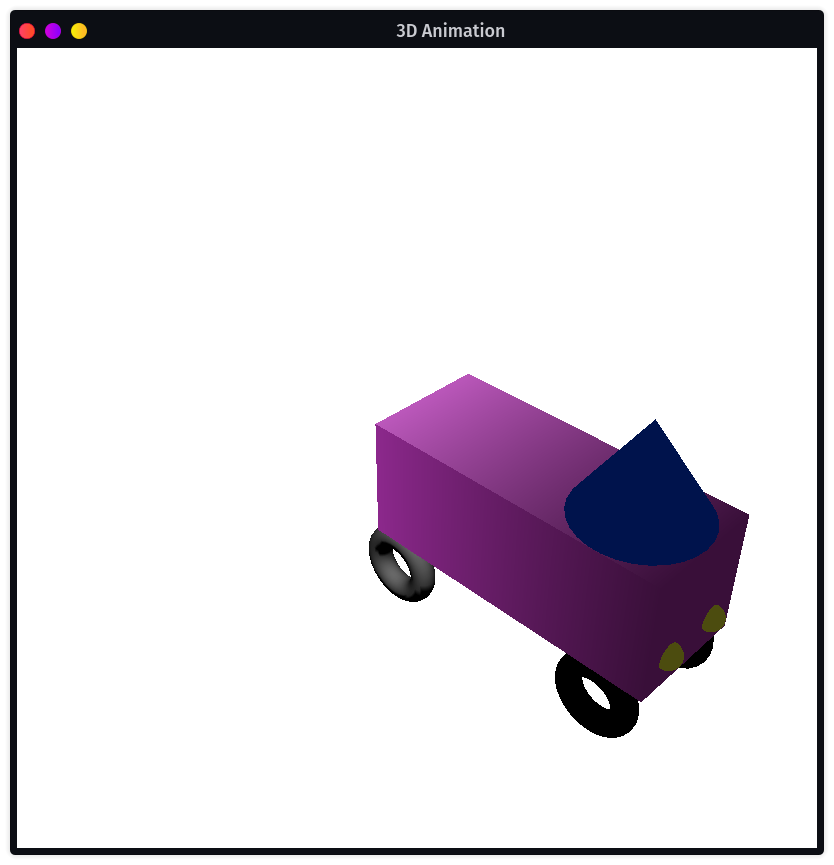
\includegraphics[height=15cm, width=15cm]{Outputs/Animation-1.png}
\end{figure}

\newpage
\subsection*{\flushleft{Output: Scene - 3}}
\begin{figure}[h]
\centering
\caption{Scene - 3.}
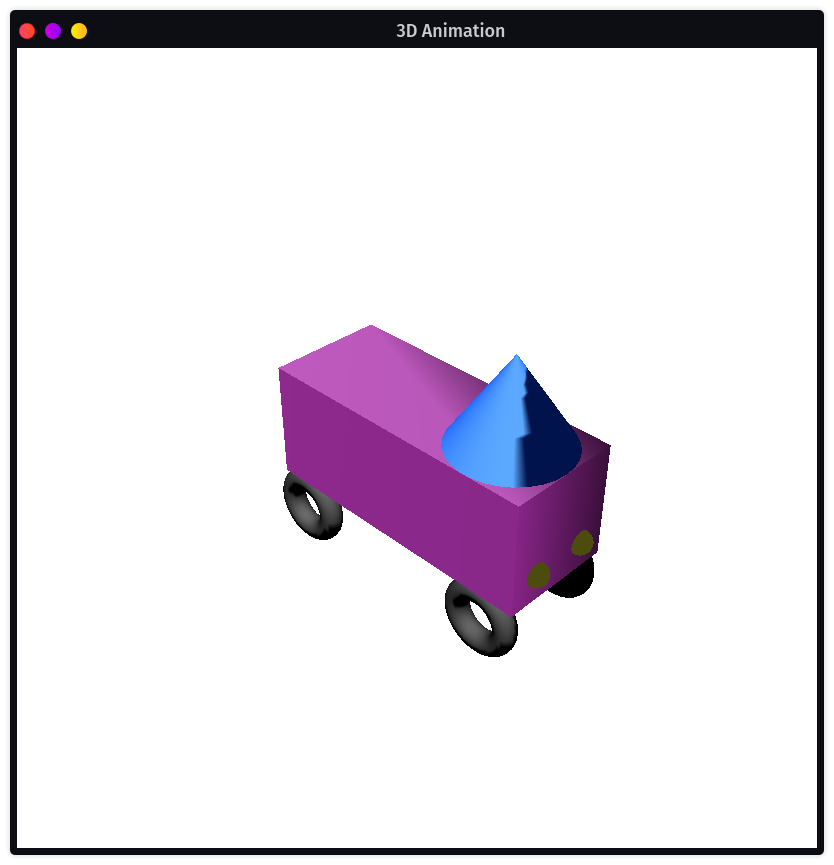
\includegraphics[height=15cm, width=15cm]{Outputs/Animation-2.png}
\end{figure}


%Learning Outcome
\newpage
\subsection*{\flushleft{Learning Outcome:}}
\begin{itemize}
\item I learnt how to use in-built 3-D object drawing methods for generating a \textbf{Torus, Cube, Cone and Sphere}.
\item I was able to apply in-built 3-D transformations to modify the objects \& position them appropriately.
\item I used these functions to draw a primitive 3D Car.
\item I understood how to set different material parameters and transformations for different objects using the \textbf{glPushMatrix() and glPopMatrix()} methods.
\item I understood how to animate the car object (perform translation) using an \textbf{FPS counter \& translation variables along the X-axis} and \textbf{glutPostRedisplay()} to redraw the scene.
\item I learnt how to define \textbf{material parameters} for \textbf{Ambient, Diffuse and Specular} components.
\item I learnt how to set-up a basic lighting model \& added \textbf{Ambient, Diffuse and Specular} components to it.
\item I implemented \textbf{spot lighting and spot directionality} for the light using \newline \textbf{GL\_SPOT\_DIRECTION \& GL\_SPOT\_CUTOFF}.
\item I was able to animate the car in and out of the lighting area.
\end{itemize}


\end{document}